\chapter{Social network boosted search ranking}

Charles Explorer is an academic search engine, which allows the user to search for publications, classes, people and study programmes in the academic domain.

The following sections, we look more into the search engine part of the application, explore the possible issues with the search results ranking, 
and experiment with utilizing the social network data for the search results ranking improvement.

\section{Full-text search}

Full-text search is nowadays an essential part of any information retrieval system. 
Many search engines - including Apache Solr in Charles Explorer - implement the full text search by utilizing the TF-IDF algorithm.
This is a simple and efficient way to rank the search results based on the relevance of the documents to the search query.

The TF-IDF algorithm is based on the term frequency and inverse document frequency of the terms in the documents - a \textit{document} is in general unstructured free text content.
Some entities in our academic search engine map well to this notion of a \textit{document} - e.g. a \texttt{publication} or \texttt{class} both have inherent textual content (titles, abstracts or syllabi).
Unfortunately, this does not hold for all the entities in the system.

As an example, a \texttt{person} entity usually does not have any explicit textual content associated with it. 
When searching for a person interested in a particular topic, the search engine has to rely on the textual content of the publications, classes, 
or other entities associated with the person, i.e. traverse - at least implicitly - the knowledge graph (or the social network of the person).

A simple solution to this problem would be to represent every person as a document, concatenating all the textual content of the entities associated with the person.
This can be further refined by assigning different weights - e.g. to the different types of entities (a \texttt{class} might be more important than a \texttt{publication}), 
or different concatenated parts of the documents (e.g. the publication title and class name are more important than the abstracts and syllabi).

Regarding adding new entities related to a given person, the concatenation also serves us well - we simply append the new entity's content to the person's document and reindex it.

However, this approach also has several drawbacks. First of all, assuming we're building a general academic search engine allowing for search in publications, classes and people, we would be indexing the same content multiple times.
This is not only inefficient in terms of storage, but also prone to update errors - there is multiple copies of the same content, which have to be updated separately.
The second issue arises from the concatenation - if any of the person's associated entities changes, the whole document has to be reindexed.
However, this might be less of a problem than the first issue, as it's not too common for academic records to get updated or removed - at least in comparison to the number of new records being added.

\subsection{Result ranking in the naive case} \label{search-ranking-issues}

Result ranking in information retrieval refers to the ordering of the search results when presented to the end user. This is often based on the relevance of the documents to the current search query.
The relevance-based ranking is often enough for the basic use case - the user is presented with the most relevant documents first, and can further explore the less relevant ones if needed.

While it might seem a bit superficial, the ranking is in fact still part of the information retrieval process. 
As multiple studies show \footnote{https://link.springer.com/article/10.1007/s11151-014-9435-y}\footnote{https://link.springer.com/article/10.1007/s10791-010-9150-8}, 
the ranking of the search results positively correlates with the click-through rate of the results 
- likely because of the typical top-left to bottom-right reading pattern of the users.
This can be further affected by other, more technical factors - such as the need for an additional user action like scroll or pagination to see the results further down the list.

%% https://link.springer.com/article/10.1007/s10791-010-9150-8 - Re-ranking search results using an additional retrieved list

Considering a simple tf-idf based search engine, the ranking of the search results is based on the relevance of the documents to the search query.
This is directly related to the term frequency of the query in the document - for a fixed query and a given document collection, we forget about the inverse document frequency, as it's constant over all the documents.
Ranking the documents solely based on the term frequency might however lead to unfavourable results - especially in the case of a proxy-representation of a given entity.


\begin{figure}[ht!]
    \captionsetup{width=.9\linewidth}
    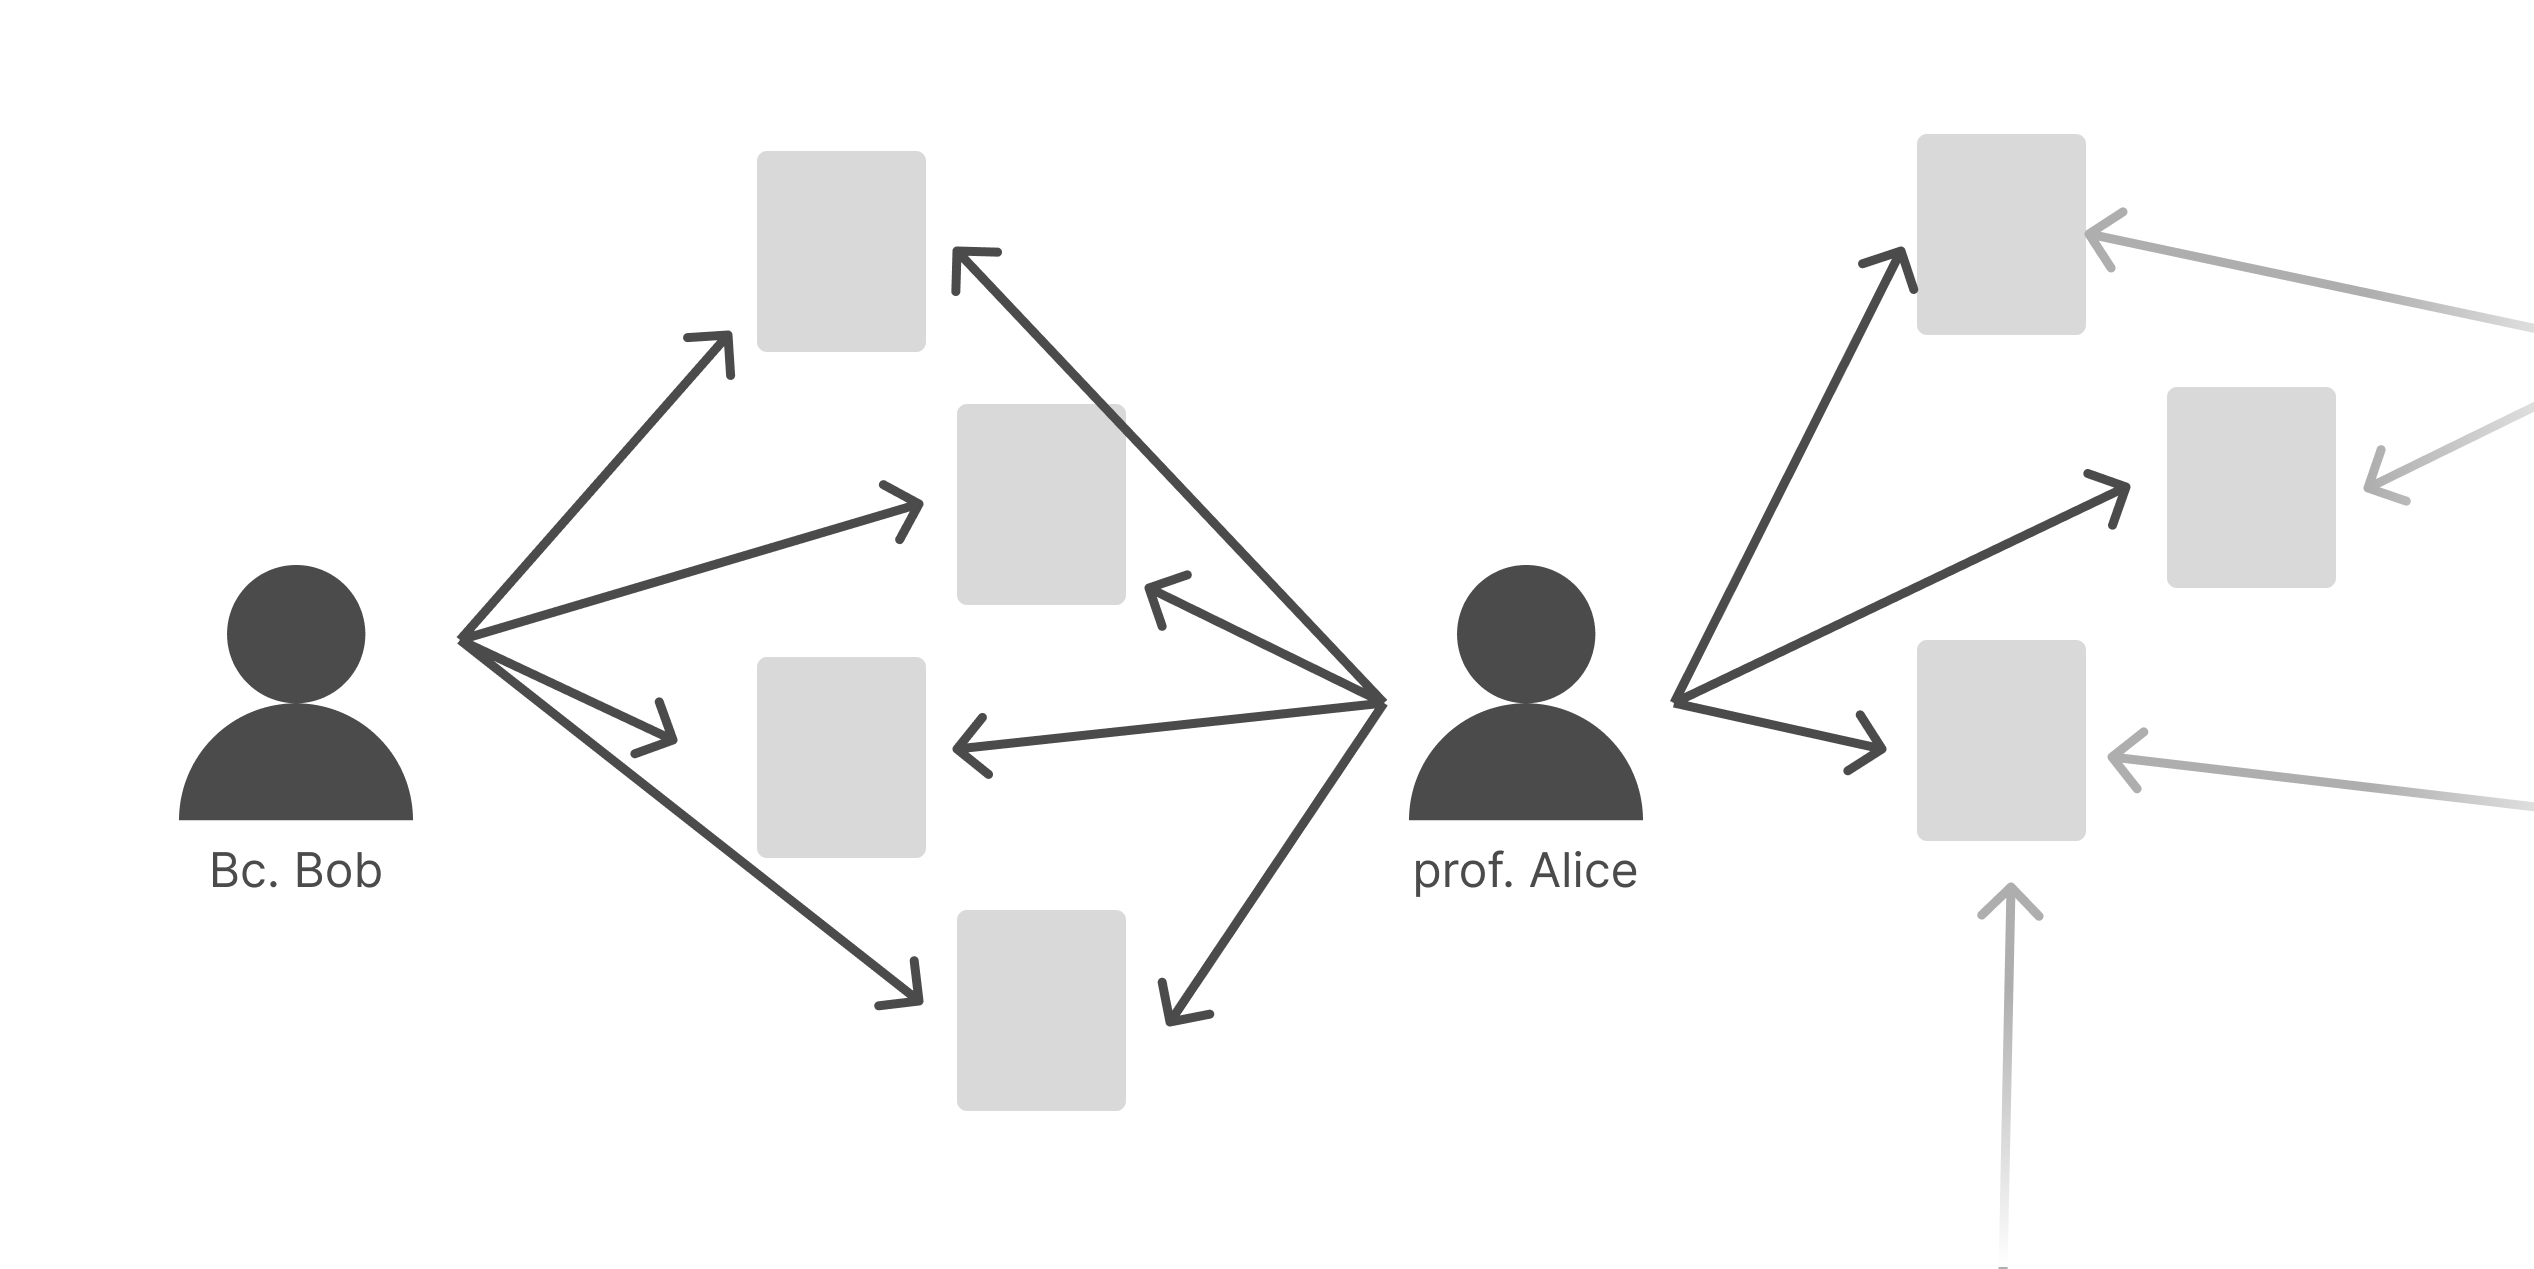
\includegraphics[width=0.8\textwidth]{../img/bob-alice-soc-netw.png}
    \centering
    \caption{Simple representation of the social network of Alice and Bob.}
\end{figure}

Let us explore the issues on an example where we represent people as documents, concatenating the textual content of the entities associated with them.
Consider two academic researchers in our system - \textit{prof. Alice} and \textit{Bc. Bob}. 
Bob is a student of Alice, and has published several papers on \textit{Information retrieval} with her. Aside from those, Bob has not published any other papers.
On the other hand, Alice has published a lot of papers on various topics - related to IR, but also to other similar fields. 
See a simple representation of their social network above.

Note that aside from the common publications, Bob has no other entities associated with him, while Alice has other publications with other co-authors.

\begin{figure}[ht!]
    \captionsetup{width=.9\linewidth}
    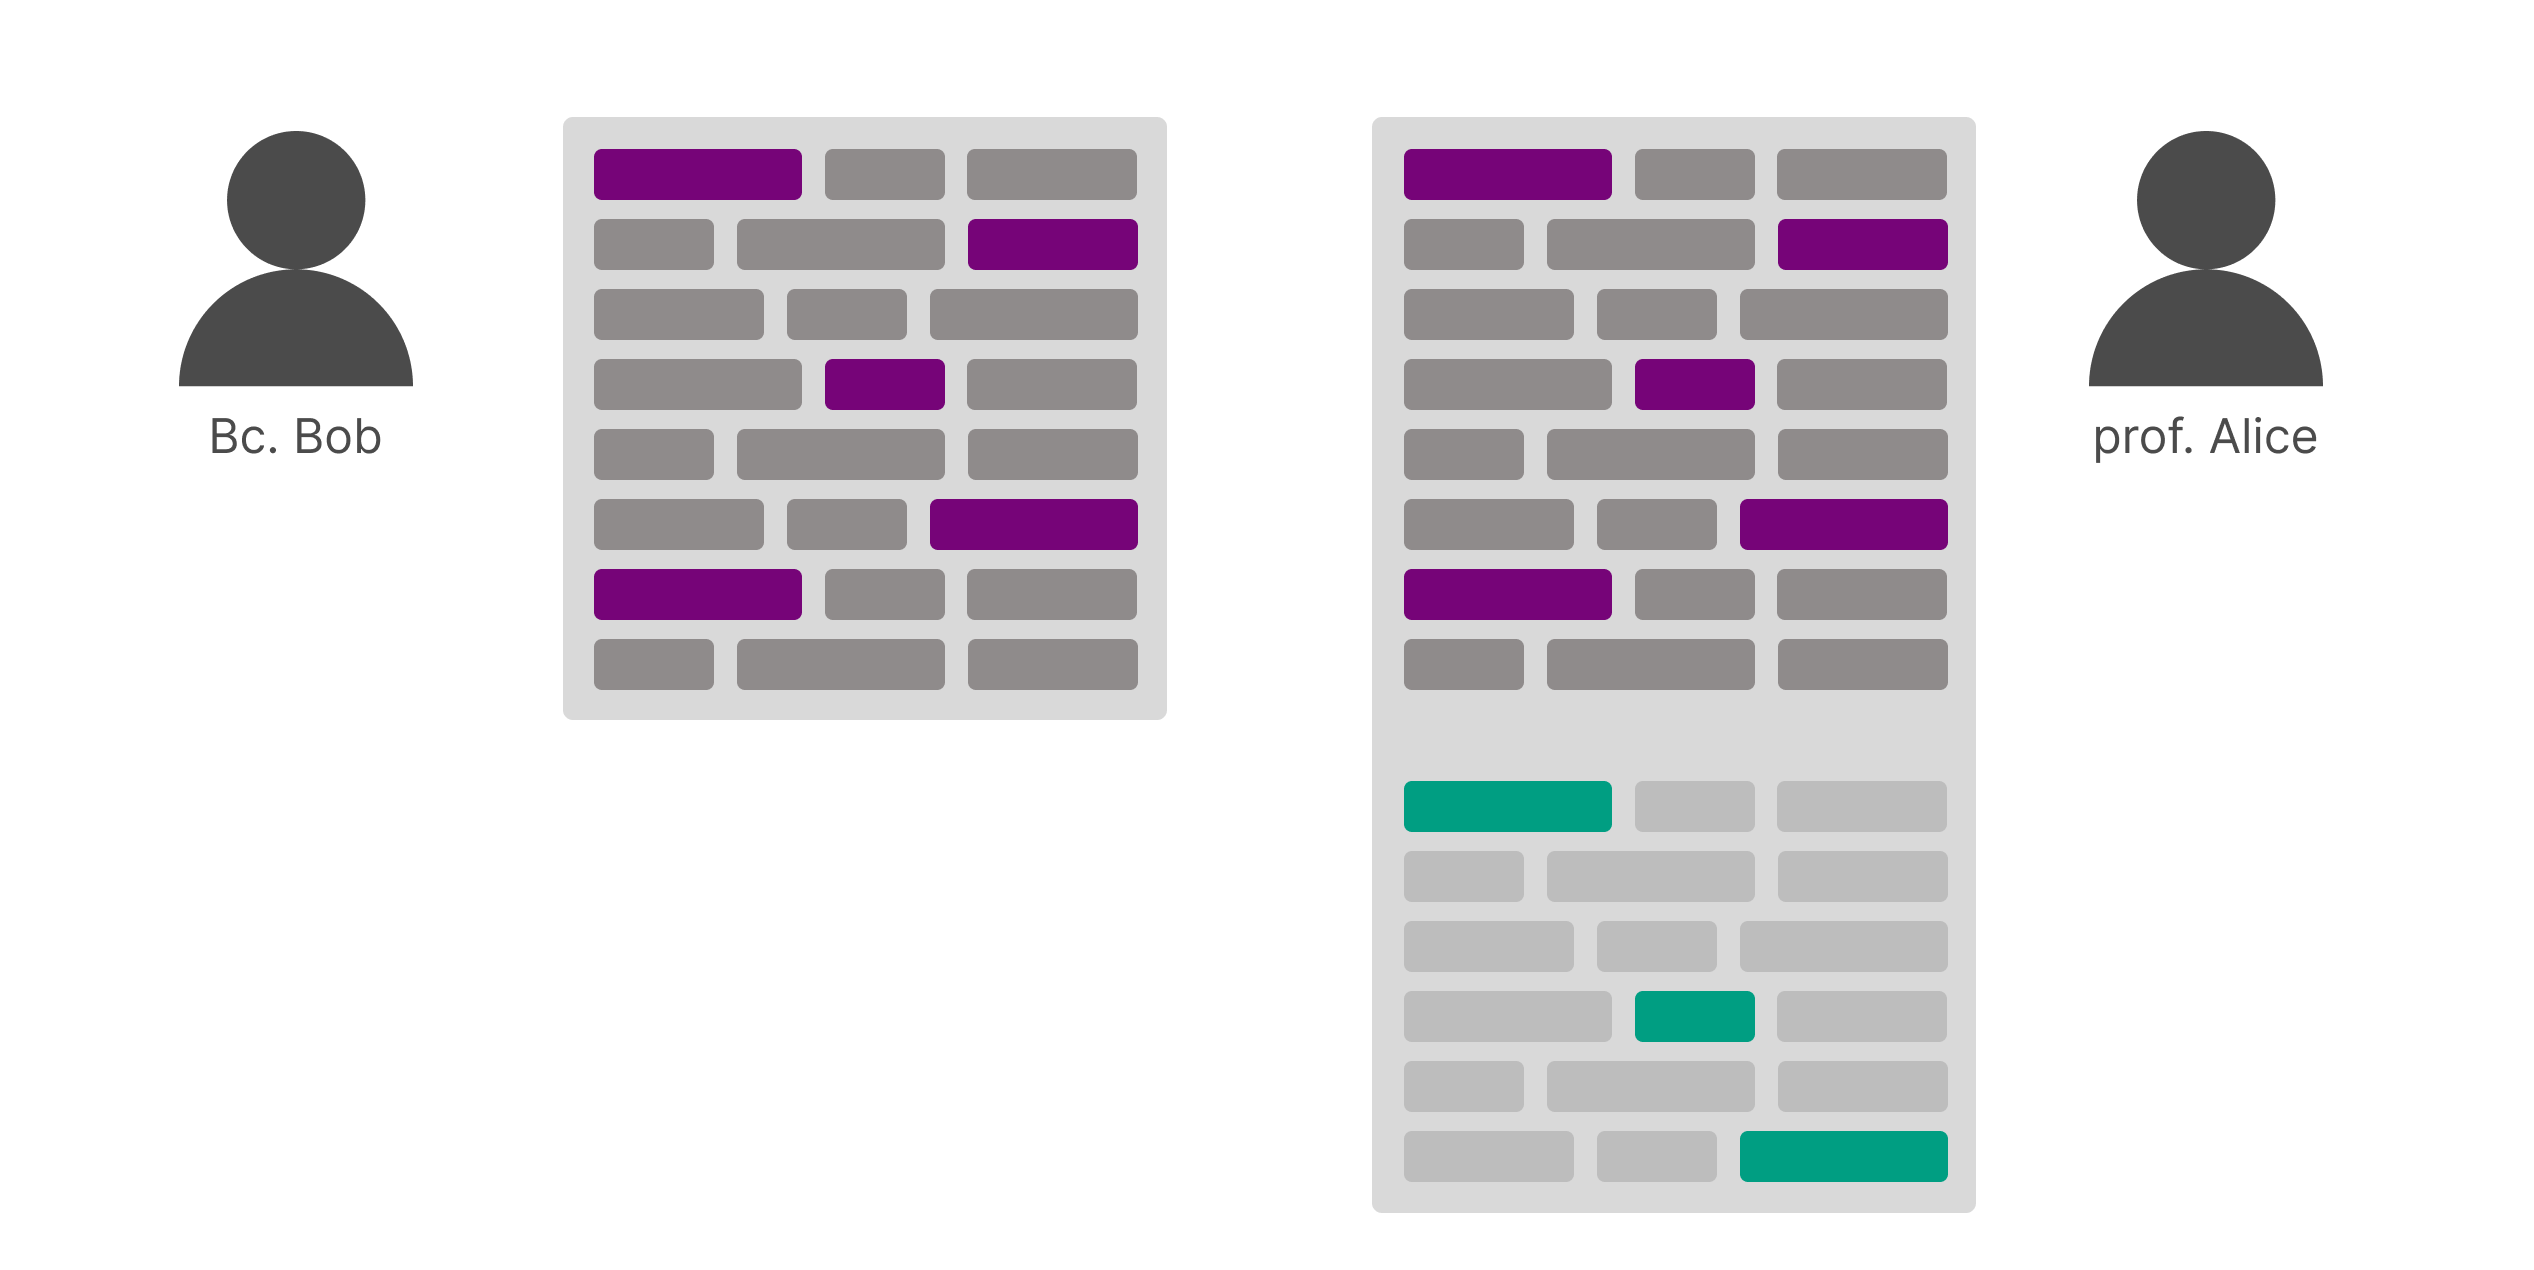
\includegraphics[width=0.8\textwidth]{../img/bob-alice-representations.png}
    \centering
    \caption{Concatenating representations of Alice and Bob as documents.}
\end{figure}

We see that the document of Bob is shorter than the one of Alice, because he has less associated entities. We also notice that the Alice's document fully contains the Bob's document.
    
The colored terms represent the current search query - if Alice only published papers on the topic of the query with Bob, the term frequency of the 
query in Bob's document would be strictly higher, because of the shorter length.
In case Alice also publishes on the topic with other co-authors, it gets harder to reason about which of the term frequencies is higher.

The relation between the tf-idf scores of the documents of Alice and Bob is expressed as follows:
\begin{subequations}
\begin{align}
\text{tf}(q, d_{\text{Bob}}) \times \text{idf}(q, D) &\stackrel{?}{>} \text{tf}(q, d_{\text{Alice}}) \times \text{idf}(q, D) \\
\text{tf}(q, d_{\text{Bob}}) &\stackrel{?}{>} \text{tf}(q, d_{\text{Alice}})
\end{align}
\end{subequations}

Normalized term frequency $\text{tf}_{q,d}$ of a term $q$ in a document $d$ is defined as the number of times the term $q$ appears in the document $d$ (denoted by $f_{q,d}$),
divided by the total number of terms in the document $d$ (the document's length).

\begin{subequations}
\begin{align}
\frac{f_{q, d_{\text{Bob}}}}{\text{len}(d_{\text{Bob}})} &\stackrel{?}{>} \frac{f_{q, d_{\text{Alice}}}}{\text{len}(d_{\text{Alice}})} \Biggm/ \;^{-1} \\
\frac{\text{len}(d_{\text{Bob}})}{f_{q, d_{\text{Bob}}}} &\stackrel{?}{<} \frac{\text{len}(d_{\text{Alice}})}{f_{q, d_{\text{Alice}}}} \Biggm/ \textit{assuming that } \mathit{f_{q, d_{\text{Bob}}} = f_{q, d_{\text{Alice}}}} \label{eq:51assumption}\\
\text{len}(d_{\text{Bob}}) \;&<\;\text{len}(d_{\text{Alice}})
\end{align}
\end{subequations}

Since we have assumed that Alice's document is a superset of Bob's document, the result inequality holds - and therefore the tf-idf score of Bob's document is higher than the one of Alice's document.

Note that the assumption in the equation \ref{eq:51assumption} is only true for the cases when Alice does not publish any other papers on the topic of the query with other co-authors.

% Because of this, the document representation of Bob will be short, compared to the one of Alice.
% Assuming the search query is \textit{Information Retrieval} - and there are no other publications or classes related to this topic in the system - 
% the search engine will consider Bob as the more relevant person for this topic. This is becuase the term frequency of the query in Bob's document is higher than in Alice's document - solely because of the length.

In either way, this approach most likely will not provide the desired outcome - while Bob has published papers only on the given topic - and therefore has higher tf-idf relevance to the query,
it is likely that Alice is the more relevant person for the searching user, since she is more experienced in the topic.

\section{Re-ranking}

In the following sections, we go over different existing re-ranking strategies utilized in other systems and explore the possibilities of using the social network data for the re-ranking in Charles Explorer.

\subsection{Existing re-ranking strategies}

In the current (2024) commercial search engines, there are often multiple re-ranking strategies available to the users.
Unfortunately, only a small portion of the engines actually discloses the details of the re-ranking algorithms used - perhaps to protect the intellectual property and the competitive advantage.

The common grounds for all those systems is the two-stage search pipeline - in the first stage, a traditional search engine is used to retrieve the initial set of results.
Then, these results are re-ranked using a different algorithm. 

While it might seem redundant, this approach allows the second algorithm to focus only the more relevant results, and be perhaps more computationally expensive.
Unfortunately, this also means that the re-ranking algorithm is not able to affect the initial search results - it can only change the order of the results.
It also brings in the issue of pagination - if the user has to go through multiple pages of the search results, the re-ranking might not be as effective,
as it only affects the current page of the results.

The re-ranking algorithms can be based on various factors - the user's previous interactions with the system, total popularity (click-through rate) of the items,
diversity of the results %link to the MMR papers https://www.google.com/search?client=firefox-b-lm&q=Maximal+Marginal+Relevance 
or NLP analysis of the documents. Especially the last one seems to be gaining traction in the recent years, as the applications of LLM models are becoming more widespread.

\subsection{Graph data-based reranking}\label{graph-based-reranking}

As we discussed in \ref{search-ranking-issues}
, the traditional tf-idf based search engine might give unsatisfactory results in the case 
of a proxy-representation of a given entity.
We might try to address this issue by utilizing the social network data for the re-ranking of the search results.

As mentioned in the previous subsection, many commercial search engines use a two-step search pipeline - the first step retrieves the initial set of results,
and the second step re-ranks them using a different algorithm. This sounds like a good fit for our problem - we use the traditional tf-idf based search engine 
to retrieve the initial set of results, and then re-rank them using the social network data. 

Only using the graph data for the search has several drawback described in the next section (\ref{graph-based-search}).

When it comes to reranking the existing search results, we utilize the social network data in several ways.

\begin{itemize}
    \item \textbf{Global node statistics}: As illustrated on the example of Alice and Bob above, 
    we can use the global statistics for the nodes in the social network to re-rank the search results. 
    These include - but are not limited to - the node degree (number of connections), centrality measures, or the number of common neighbours.

    Such statistics can be precomputed for every node in the social network before the search and stay constant over all the search queries.

    \item \textbf{Query relevant node statistics}: Unlike the global node statistics, query-relevant node statisics are computed only for the nodes in the search results.
    
    These can perhaps define the node's relevance better (e.g. the number of query-relevant publications connected to a given person), but are often more computationally expensive to compute.
    Given the variability of the queries, it is also harder (or impossible) to precompute these statistics.
\end{itemize}

%% todo structure
\subsection{Graph data-based search} \label{graph-based-search}

It would also be possible to use the social network data to entirely replace the concatenated person representations in the search engine - we could 
only search through the ``first-order entities'' (i.e. classes and publications) and then query the social network graph for the people associated 
with the results of the search. 

This approach has several drawbacks - aside from the questionable performance and scalability / developer effort, it also might not be as effective as the concatenated representation.

With the concatenated approach, we have to retrieve only \textasciitilde{} 30 results (people) for every page of the search results. 
Those are also already ranked by the relevance to the query - even though this might not be perfect, the tf-idf based ranking is still a good approximation.

With the proposed graph-based approach, we would have to retrieve many more publications and classes on each search - note that we are no longer 
looking for the most-relevant class or publication, but for the most-relevant person - which is rather an aggregation of the relevance of the associated entities.
This might lead to a lot of unnecessary data retrieval and processing and become the bottleneck for the possible applications built on such data.


\section{Benchmarks}

To determine the performance of our proposed re-ranking solution, we establish benchmarks to compare the results of the traditional tf-idf based search engine with the social network enhanced search engine.

The common denominator for many of the ranking measures - like discounted cumulative gain or mean reciprocal rank - is the \textit{user interaction}.
The user is presented with the search results and picks the most relevant one or scores the results based on the relevance to the query.

Unfortunately, this is not applicable to our case - while we are tracking the user interactions in the Charles Explorer web appplication, the amount of collected data is far too low to be statistically significant.

\begin{mybox}{}
    The following section is described in greater detail in my blog posts series \textit{Benchmarking Charles Explorer search result rankings}\footnote{\url{https://jindrich.bar/edu/thesis-blog/}}.
    
    The blog posts contain the detailed description of the process of collecting the search queries for the benchmarking of the search results ranking in Charles Explorer.

    Since the blog posts are rendered Jupyter notebooks, they also contain the code snippets used for the data collection and analysis.
    The implementation of all the steps - i.e. data collection, data preprocessing, and the benchmarking itself - is fully reproducible and available in the embedded code snippets.
\end{mybox}

To establish a gold standard for the search results relevance, we do not have to rely solely on human interactions.

Elsevier Scopus\footnote{https://www.elsevier.com/products/scopus} is a large academic database, which provides a search engine for the academic publications.
Aside from the web application, it also provides a REST API for consuming the data programmatically.

We use the Scopus API to retrieve ranked lists of publications for a given query, and then use the ranking of the publications as the source of the ``global relevance'' for the search query in the benchmark.
Simply put, by comparing the (ranking of the) search results in our search engine to the results of the Scopus search engine, we determine the relevance of the search results.

We are expecting the search results of the Scopus search engine to be more precise and relevant than the ones of the Charles Explorer search engine -
Scopus is a commercial product with a large team of developers and researchers, while Charles Explorer is a small academic project.
The data available to scopus also contain details about the citations of the publications and author profiles, which can be used to further improve the search results ranking.

\subsection{Sampling the search query set}

As the first step, we need to sample the \textit{search query set} for the benchmark. 
Since we want to rule out possible biases - or at least mitigate their impact - we need a large and diverse enough set of queries to compare the search engines on.

Generating these manually would be time-consuming and error-prone. 
Therefore, to solve this issue, we use a \textit{wordnet} - a lexical language database of English.
We use it to generate a large set of diverse queries, perhaps less biased than a manually generated set.

We start by selecting a set of \textit{seed words} - in our experimental case, those were the words \textit{``field of study''} and \textit{``medicine''}.
Then, we traverse the wordnet to recursively find the hyponyms of those seed words, up to a certain depth.

Running this process for the seed words \textit{``field of study''} and \textit{``medicine''} with the depth of 4, we get a set of \texttt{915} search queries.

While this approach gives us a sizable set of queries, we have no guarantee of the quality of the queries - they might be too general or too specific, or not relevant to the academic domain at all.
One of our goals was also to ensure the fairness of the query set - this is not guaranteed by the wordnet traversal either, as the queries might be too similar to each other (or target the similar topics in the publications).

\subsubsection{Ensuring the query set fairness}

While \textit{fairness} is a largely subjective measure, we let the available data guide us in this case.
For the \textit{academic publications}, we have their \textit{titles}, \textit{abstracts}, \textit{keywords}, \textit{faculty affiliations} and \textit{authors} avaialble in our system.

Since titles, abstracts and keywords are free text fields, we omit them from our analysis - the preprocessing of the text data is a complex task on its own.
Given the nature of our experiment - i.e. measuring the impact of using the social network data for the search results ranking - we have to leave the authorship information out as well.

This process leaves us with the faculty affiliations.

Charles University has \textit{17} faculties, each with a different focus and research areas.
Each publication in our data is attributed to exactly one faculty.
This allows us to use the faculty affiliations as a proxy for the fairness of the search queries.

\textbf{Kullback-Leibler divergence}

As the fairness measure, we compare the distribution of the faculty affiliations in the search query results 
to the distribution of the faculty affiliations of all the publications in the system.

The standard way of comparing probability distributions is the \textit{Kullback-Leibler divergence} - a measure of how one probability distribution diverges from a second, expected probability distribution.

For discrete probability distributions $P$ and $Q$ defined on the same sample space $\Omega$, the Kullback-Leibler divergence from $Q$ to $P$ is defined as

$$
D_{KL}(P||Q) = \sum_{\omega \in \Omega} P(\omega) \log \frac{P(\omega)}{Q(\omega)}
$$

The KL-divergence is always non-negative, and is zero if and only if $P$ and $Q$ are the same distribution.

With the measure of the fairness of the search query set established, we now proceed to the benchmarking of the search results ranking in Charles Explorer.

By sampling up to 30 results for each search query from the Charles Explorer search engine, we acquire the faculty distribution for the entire search query set ($N = 915$).
We then compare this distribution to the distribution of the faculty affiliations of all the publications in the system.

\begin{figure}[ht!]
    \captionsetup{width=.9\linewidth}
    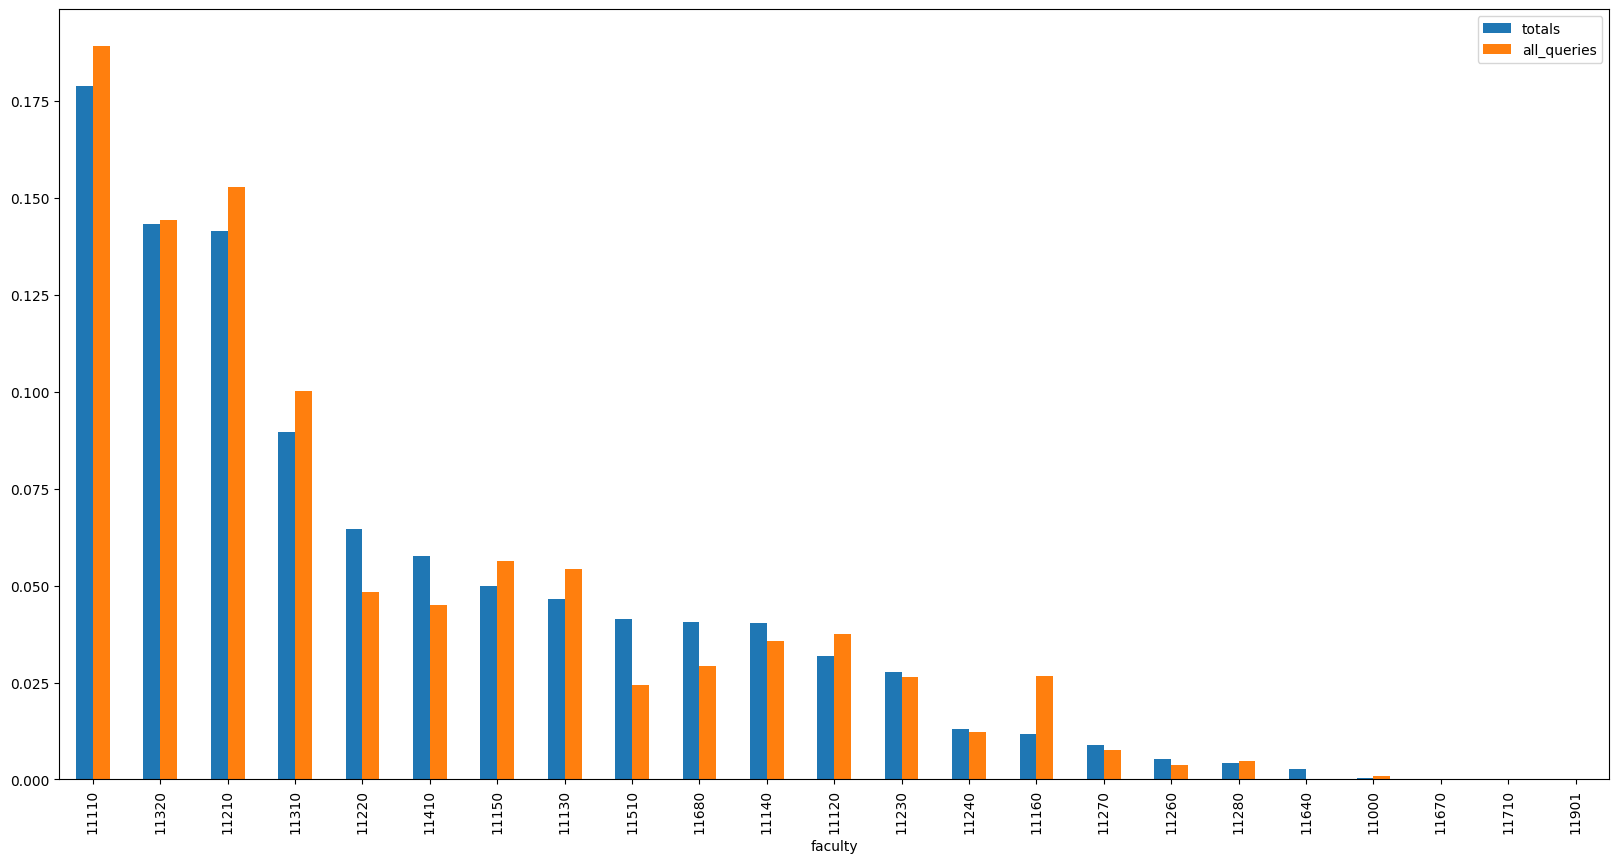
\includegraphics[width=0.8\textwidth]{../img/all-queries-vs-totals.png}
    \centering
    \caption{Comparing the faculty distribution of the search query results \textit{(orange, right)} to the distribution of all the publications in the system \textit{(blue, left)}.}
\end{figure}

The Kullback-Leibler divergence of the faculty distribution of the \textbf{search query results} from the distribution of \textbf{all the publications} in the system is approximately \texttt{0.0471}.

\textbf{Optimizing the KL-divergence}

With the defined measure of the fairness of the search query set, we now try to optimize it.
In our case, optimizing the KL-divergence means \textit{finding a subset} of search queries which would minimize the divergence of the faculty distribution of the search query results from the distribution of all the publications in the system.

Unfortunately, this poses serious challenges. 
Finding a subset with an optimal aggregate property is a well-known NP-hard problem - often referred to as the \textit{0-1 knapsack problem} or the \textit{subset sum problem}.
Even worse, we cannot simply reuse some of the existing algorithms for these problems, as those rely on the distributivity and associativity of the sum operation. 
This is however not the case for the KL divergence.

Similarly to the sum of the item values (in the Knapsack problem), the KL divergence is evaluated on the entire set, but unlike the sum, the items themselves do not have any “value” - and their contribution to the KL divergence changes depending on the other items in the set. 
This leaves us with a limited choice of algorithms to solve the problem. 
Because of the complexity of the problem and its smallish role in this work, we use a simple random search. 

This approach works in two steps:

%% todo pseudocode algorithm for the optimization
\begin{enumerate}
    \item Repeatedly sample a random subset of size $k$ of the search queries, keeping track of the subset with the lowest KL divergence.
After a fixed number of iterations, take the subset with the lowest KL divergence.
    \item From the $k$-sized subset, repeatedly remove the search query with the highest contribution to the divergence.
Stop when the KL-divergence stops decreasing, i.e. we cannot remove any more search queries to decrease the divergence, or we've reached the minimum subset size $l$.
\end{enumerate}

This is a simple and computationally cheap approach, but it might not always find the optimal solution.
Furthermore, since the KL-divergence is a non-convex function, the second step of the algorithm might get stuck in a suboptimal solution.
While this could be mitigated using a more complex optimization algorithm (e.g. simulated annealing etc.), experimental results show that the simple random search is sufficient for our purposes.

\begin{figure}[ht!]
    \captionsetup{width=.9\linewidth}
    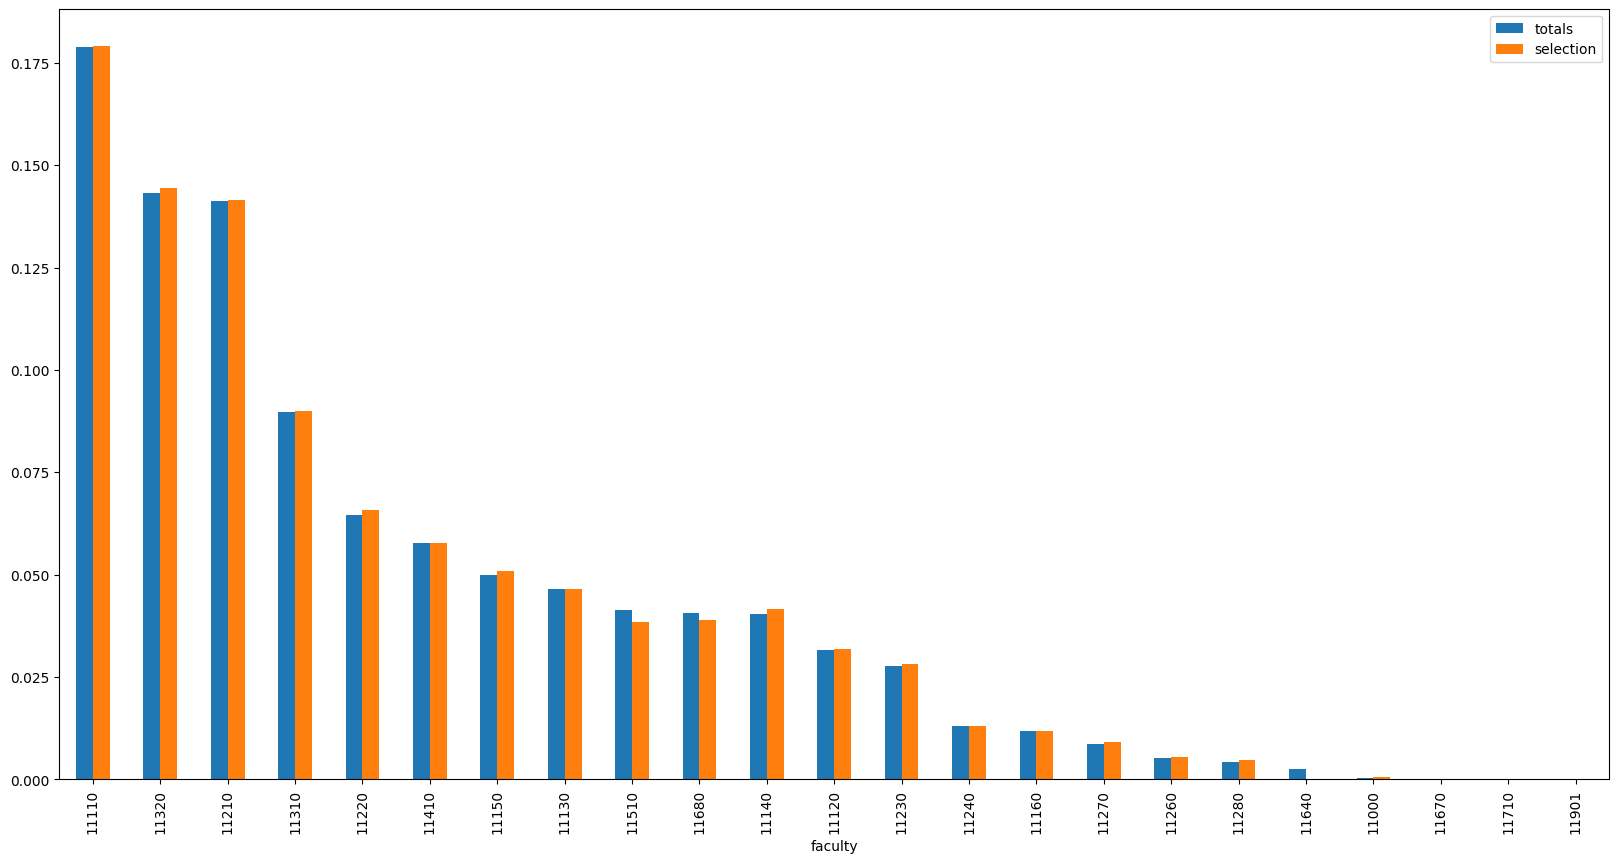
\includegraphics[width=0.8\textwidth]{../img/all-queries-vs-totals-corrected.png}
    \centering
    \caption{Comparing the faculty distribution of the search query results \textit{(orange, right)} to the distribution of all the publications in the system \textit{(blue, left)} \textit{after running the optimization algorithm}.}
\end{figure}

Running the optimization algorithm with $n = 10000$ initial random samples of size $k = 300$ on the search query set, we arrive at a set of $174$ queries with the search result KL-divergence of \texttt{0.00317}. 
This is a significant improvement over the original divergence of \texttt{0.0471} and we will consider this a fairer subset of the search queries for the benchmarking.

\subsection{Collecting the data}

Since our proposed benchmark only evaluates the search results ranking, we collect the search results for the benchmark queries in advance.
Similarly, we also collect the data from the Scopus API for the same queries, as the automated relevance feedback.

While collecting the search results from the Charles Explorer search engine is straightforward since the API is available to us, 
the Scopus Advanced search feature requires us to use a special query language\footnote{\url{https://schema.elsevier.com/dtds/document/bkapi/search/SCOPUSSearchTips.htm}} to submit the search queries. 
This query language offers a set of Prolog-like functors, 
each related to a specific field - or a set of fields - of the publication record. 
The attributes of these functors are used in a \textit{substring search} on the specified fields.

Apart from this, the query language also supports logical operators, such as \texttt{AND}, \texttt{OR}, and \texttt{AND NOT}.

We will use two of the available functors: \texttt{TITLE-ABS-KEY} and \texttt{AF-ID}:

\begin{itemize}
    \item \texttt{TITLE-ABS-KEY} searches for the specified substring in the title, abstract, and keywords of the publication record. 
    In this regard, it is similar to the full-text search in Charles Explorer, which searches in the same fields.
    \item \texttt{AF-ID} filters the search results by the organisation affiliation of the publication. This is useful for filtering the search results to only those publications where at least one of the authors is affiliated with Charles University. Since Elsevier Scopus contains many records not affiliated with Charles University (but Charles Explorer only contains such records), this will help us to get a more comparable sets of search results.
\end{itemize}

By calling the Scopus API, we get the search results in JSON format, which we then process and store in our database for the benchmarking.

\begin{figure}[ht!]
        \scriptsize
        \centering
        \begin{tabular}{|l|l|l|l|l|l|l|}
        \hline
            ~ & ranking & totalAuthors & scopusId & pubYear & citationCount & referenceCount \\ \hline
            ranking & 1.000000 & 0.038005 & 0.081229 & 0.109848 & 0.062467 & 0.053487 \\ \hline
            totalAuthors & 0.038005 & 1.000000 & 0.033948 & 0.040538 & 0.113336 & 0.094358 \\ \hline
            scopusId & 0.081229 & 0.033948 & 1.000000 & 0.806411 & 0.015393 & 0.243830 \\ \hline
            pubYear & 0.109848 & 0.040538 & 0.806411 & 1.000000 & 0.033019 & 0.283521 \\ \hline
            citationCount & 0.062467 & 0.113336 & 0.015393 & 0.033019 & 1.000000 & 0.218415 \\ \hline
            referenceCount & 0.053487 & 0.094358 & 0.243830 & 0.283521 & 0.218415 & 1.000000 \\ \hline
        \end{tabular}
    \caption{Correlation matrix of the Elsevier Scopus search results numeric attributes.} 
\end{figure}

We see that the \texttt{ranking} column - the position of a publication in the search results - is only very weakly correlated with the other numeric attributes of the search results.
This suggests that the default Scopus ranking is mostly influenced by the full-text search and does not take much reranking into account.

It also suggest that the Scopus result ranking might not be too dependent on the social network measures and that we might not be able to improve the ranking 
by using the social network data (as the ``explicit'' social network data like the citation count or the reference count are not correlated with the ranking).

\subsection{Calculating baseline values}

With the data collected, we now proceed with the actual analysis of the search results ranking in Charles Explorer.

Considering the Scopus search results as the gold standard, we calculate the per-query precision, recall and $F_1$ score for the search results of Charles Explorer.

\begin{figure}[!ht]
    \captionsetup{width=.9\linewidth}
    \centering
    \begin{tabular}{|l|l|l|l|}
    \hline
        \textbf{Query} & \textbf{Precision} & \textbf{Recall} & \textbf{$F_1$ score} \\ \hline
        physics & 0.043011 & 0.040000 & 0.041451 \\ \hline
        bolus & 0.125000 & 0.121212 & 0.123077 \\ \hline
        draft & 0.010870 & 0.010753 & 0.010811 \\ \hline
        $\hdots$ & $\hdots$ & $\hdots$ & $\hdots$ \\ \hline
    \end{tabular}
    \caption{Per-query precision, recall and $F_1$ score for the search results of Charles Explorer.}
\end{figure}

After aggregation over all the queries, this gives us the following unfavourable statistics:

\begin{figure}[!ht]
    \captionsetup{width=.9\linewidth}
    \centering
    \begin{tabular}{|l|l|}
    \hline
        Mean & 0.208727 \\ \hline
        Standard deviation & 0.211699 \\ \hline
        Minimum & 0.010101 \\ \hline
        25\% & 0.074786 \\ \hline
        50\% & 0.137028 \\ \hline
        75\% & 0.265263 \\ \hline
        Maximum & 1.000000 \\ \hline
    \end{tabular}
    \caption{Aggregated statistics of the $F_1$ score for the search results of Charles Explorer.}
\end{figure}

We see that the current Charles Explorer search results differ quite a lot from the Scopus search results. 
This can be caused by mutiple reasons - either the publications are not present in the Scopus database, or the queries are not specific enough - and the search results are returning partially disjoint sets of publications.

Note that this is an issue that goes beyond re-ranking the Charles Explorer search results. 
We cannot quantify the benefit of reordering the search results if we consider all the search results irrelevant.
This hinders our ability to use the Scopus search results ranking as the proxy for the relevance feedback.

Since this thesis is focused on the search result ranking algorithms, we will proceed with the benchmarking as planned. 
However, to improve the relevance score assignment, we add a \textit{similarity search} step. 
 
In the $F_1$ score calculation, we are only matching the Charles Explorer search results with the Scopus search results by the publication title (case-insensitive). 
This matching criterion is prone to even the slightest variations in the publication titles, which can lead to false negatives.

\subsubsection{Inferring the publication relevance with semantic search}\label{semantic-search}

In the proposed \textit{similarity search} step, we use the similarity of LLM (Large Language Model) embeddings to match the publication titles. 
This should help us to relate the publications missing from the Scopus search results to the ones present there and assign them a relevance score.

\begin{mybox}{LLM embeddings}

    \textit{LLM embeddings} are vector representations of a given text, generated by a large language model.
    While those can be arbitrary vectors, embeddings are usually optimized to capture the semantic meaning of the text. 
    
    This means that texts with similar meanings should have similar embeddings - i.e. the (cosine) similarity of the embedding vectors should be high.
\end{mybox}

We enhance the relevance calculation with the similarity search process as follows:

\begin{enumerate}
    \item By the means of an \textit{LLM embedding model}, we precalculate the embeddings for the publication titles of the Elsevier Scopus search results. 
    We store these embeddings in a vector database.
    \item For each publication title in the Charles Explorer search results, we calculate its embedding. 
    In the database, we search for the nearest embedding among Scopus search results embeddings. 
    Futhermore, we require the retrieved document to be a result of the same query (in Elsevier Scopus) as the Charles Explorer search result.
    \item We calculate Charles Explorer document’s inferred relevance from the most similar document’s attributes - e.g. its position in Scopus search.
\end{enumerate}

For the document embedding, we use the \texttt{all-MiniLM-L6-v2}\footnote{\url{https://www.sbert.net/docs/sentence_transformer/pretrained_models.html}} sentence - transformer model. 
This is a general-purpose English embedding language model designed for running on consumer-grade hardware. 
Due to its small size and competitive performance, it’s often used for the real-time use-cases, like semantic search or RAG (Retrieval-Augmented Generation).

For the similarity search on the embeddings we use the ChromaDB database\footnote{\url{https://www.trychroma.com/}}. 
ChromaDB is a vector database designed for the similarity search on the embeddings, with support
for enhancing the search results with the additional metadata attributes of the documents.

\newpage

\begin{figure}[ht!]
    \captionsetup{width=.9\linewidth}
    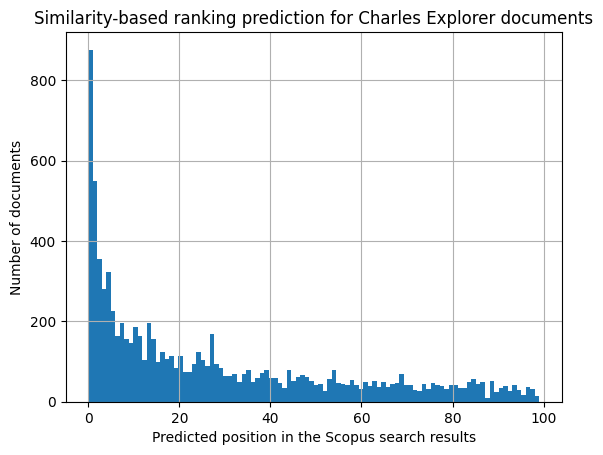
\includegraphics[width=0.8\textwidth]{../img/llm-embedding-positions-hist.png}
    \centering
    \caption{Histogram of inferred positions of the Charles Explorer search results in the Scopus search results.}
\end{figure}

This process gives us the predicted rankings which follow a rather skewed distribution. 
However, this does not pose a serious problem to our benchmark.

Firstly, we are not trying to predict the exact ranking of the search results, but rather to assign a relevance score to each search result. 
The peak of the distribution is at the top of the rankings, 
which is in line with the well known tendency of human users 
to have much clearer opinion about the few top results than the long tail of the search results (\cite{9357332}).

Secondly, the left-skewed distribution might be caused by non-uniform lengths of the search result lists. 
Since for some of the queries, Scopus returns only a few relevant search results (100 is only the maximum limit), 
the resulting predicted rankings will be skewed towards the top of the list for these queries.

\subsection{Calculating the base nDCG}

Using the original ranking positions and the predicted ranking positions as the source for the 
relevance feedback, we calculate the \textit{nDCG} (Normalized Discounted Cumulative Gain) score for the 
search result ranking.

DCG score for a single search result list is calculated as the sum of the relevance scores of the search results, discounted by their position in the ranking.

$$
DCG_\text{list} = \sum_{i=1}^{N} \frac{2^{rel_i} - 1}{\log_2(i + 1)}
$$

The IDCG score is the DCG score of the ideal ranking of the search results, i.e. the items in the list are sorted in descending order by $rel_i$.

Normalized DCG score is then calculated as the ratio of the DCG score to the IDCG score.

$$
nDCG_{\text{list}} = \frac{DCG_\text{list}}{IDCG_\text{list}}
$$

To transform the predicted Scopus rankings from \ref{semantic-search} into relevance feedback, 
we introduce a new function $rel_q(d)$.

For a given query $q$, the document $d$ is considered to have relevance of $rel_q(d)$, 
which is \textit{inversely proportional} to its predicted ranking. 
This is necessary for the \textit{nDCG} score calculation, which requires more relevant documents 
to have higher relevance scores.

The inverse proportionality is achieved by the following formula:
\[rel_q(d) = \frac{a}{\text{rank}_q(d) + 1}\]

where $a$ is a constant that scales the relevance scores and can help achieve better 
stability of the nDCG score with respect to rounding errors.

For the purpose of the experiments in this thesis, we set $a = 5$. 
The $+1$ in the denominator is necessary to avoid division by zero, as our rankings are $0-$based.

While it would be possible to achieve the ranking $\rightarrow$ relevance transformation via e.g. subtracting the predicted ranking from the total number of search results, 
our proposed method with $rel_q(d)$ introduces a \textit{non-linear} transformation of the predicted rankings. 
This differentiates better between the search results that are ranked higher in the Scopus search results. 
This is again in line with the beforementioned tendency of the human users to have clearer opinions about the top search results.

nDCG calculation over the search results of Charles Explorer with the predicted relevance scores from \ref{semantic-search} gives us the following results:

\begin{figure}[!ht]
    \captionsetup{width=.9\linewidth}
    \centering
    \begin{tabular}{|l|l|l|l|}
    \hline
        ~ & dcg & idcg & ndcg \\ \hline
        mean & 14.919819 & 19.167405 & 0.761607 \\ \hline
        std & 16.810894 & 17.665142 & 0.180979 \\ \hline
        min & 0.094340 & 0.094340 & 0.405669 \\ \hline
        25\% & 5.250473 & 7.704989 & 0.627563 \\ \hline
        50\% & 9.527864 & 14.840570 & 0.736246 \\ \hline
        75\% & 18.064385 & 24.112511 & 0.934206 \\ \hline
        max & 104.693354 & 104.693354 & 1.000000 \\ \hline
    \end{tabular}
    \caption{Aggregated statistics of the nDCG score for the original search results of Charles Explorer (\textit{query count = $149$}).}
\end{figure}

The mean nDCG score of $0.761607$ suggests that the search result ranking in Charles Explorer already works well - and that the relevance feedback based on the predicted Scopus rankings gives us a good approximation of the relevance of the search results.

\subsection{Using graph metrics for re-ranking}

With the relevance feedback and baseline benchmark values established, we can now proceed with the re-ranking of the search results in Charles Explorer using the social network data.

Due to the large size of the social network %%( todo number of nodes + edges)
we prefer to use local graph statictics - or \textit{query relevant} statistics, as defined in \ref{graph-based-reranking}.

\subsubsection{Ego betweenness centrality}\label{ego-betweenness}

The “betweenness centrality” is a graph node measure that quantifies the importance of a node in a graph. 
It is calculated as the number of shortest paths between all pairs of nodes that pass through the node in question:

\[g(v) = \sum_{s \neq v \neq t} \frac{\sigma_{st}(v)}{\sigma_{st}}\]

where $s$, $t$ and $v$ are nodes in the graph, $\sigma_{st}$ is the number of shortest paths between nodes $s$ and $t$, and $\sigma_{st}(v)$ is the number of shortest paths between $s$ and $t$ that pass through $v$.

While this is usually calculated in the context of the entire graph, it is an useful measure for ego-networks too, as it can help us quantify the importance of a node in its local neighbourhood. 
\cite{egonetworkbetweenness} have shown that for real-life networks, the ego betweenness centrality often correlates with the actual global betweenness of a node in the graph.

In our data, the collaboration graph is bipartite - the nodes are either publications or people and there are no edges between the nodes of the same type.
This means that the ego betweenness centrality of a publication is in fact proportional to the number of people that have collaborated on the publication.

\subsubsection{2-hop betweenness centrality}
Similar to the \ref{ego-betweenness}, we calculate the 2-hop betweenness centrality as the betweenness centrality of a node 
in a subgraph induced by the node and its 2-hop neighbourhood.

In our case of the bipartite collaboration graph, the 2-hop betweenness centrality of a publication is no longer proportional only to the number of people that have collaborated on the publication,
but also to the number of other publications that the people have collaborated on.

Note that this concept can be further extended to the $k$-hop betweenness centrality, but the computational complexity of the centrality calculation grows exponentially with the $k$.
Materializing the induced subgraphs for the $k$-hop betweenness centrality calculation also poses a challenge in regard to the memory consumption. 

In our experiements, we only use the $1-$ and $2-hop$ betweenness centrality as the query-relevant node statistics.